\documentclass[a4paper,12pt]{report}
% \usepackage{styles/fbe_tez}
\usepackage[utf8x]{inputenc} % To use Unicode (e.g. Turkish) characters
\renewcommand{\labelenumi}{(\roman{enumi})}
\usepackage{amsmath, amsthm, amssymb}
 % Some extra symbols
\usepackage[bottom]{footmisc}
\usepackage{cite}
\usepackage{url}
\usepackage{graphicx}
\usepackage{longtable}
\graphicspath{{figures/}} % Graphics will be here

\usepackage{multirow}
\usepackage{subfigure}
\usepackage{algorithm}
\usepackage{algorithmic}

\begin{document}

% Title Page
\title{CMPE 492 \\ Stablecoin Flow Analysis on Blockchains}
\author{
Celil Özkan \\
\\ \\
Advisor: \\ 
Can Özturan
}
\date{\today}
\maketitle{}
\pagenumbering{roman}
\tableofcontents

\chapter{INTRODUCTION}
\pagenumbering{arabic}


\section{Broad Impact}

Stablecoins have become a critical infrastructure component in digital finance. They are widely used for cross-border settlement, centralized exchange (CEX) operations, decentralized exchange (DEX) liquidity provision, lending protocols, and cross-chain bridge transfers. As stablecoin activity spans multiple blockchain networks, understanding how value flows and which entities act as major hubs is important for both technical and economic analysis.

This project focuses on extracting ERC-20 transfer events for selected stablecoins from EVM-compatible networks and building a data foundation for graph-based flow analysis. The implemented system provides a scalable and reproducible pipeline for collecting and storing large-scale blockchain data, enabling further analysis without relying on proprietary or closed datasets.

The broader impact of this work extends beyond engineering. By making transaction flow data more accessible and analyzable, the system can support research in financial transparency, systemic risk analysis, and regulatory insight into digital asset ecosystems.

Potential impact areas include:
\begin{itemize}
\item Measuring concentration of liquidity and systemic dependency on specific protocols.
\item Identifying major transfer corridors between users, exchanges, bridges, and protocol contracts.
\item Supporting transparent research on cross-network asset movement.
\item Providing a practical educational pipeline for blockchain data engineering.
\end{itemize}

Overall, this project contributes to improving the observability and understanding of decentralized financial systems, which is increasingly important as these systems continue to grow in scale and influence.

\section{Ethical Considerations}

This project uses only publicly available on-chain data, including transaction logs and metadata. No attempt is made to deanonymize blockchain addresses or associate them with real-world identities. Address classification, when applied, is limited to high-level categories such as exchanges (CEX), decentralized protocols (DEX), bridges, or generic user accounts, without identifying individual persons.

Despite relying on public data, several ethical considerations arise:

\begin{itemize}
\item \textbf{Misclassification risk:} Address labels (e.g., CEX, DEX, bridge) may be incomplete or outdated, leading to incorrect interpretations.
\item \textbf{Attribution risk:} A single wallet address may represent multiple actors or automated systems, so behavioral conclusions must remain probabilistic rather than definitive.
\item \textbf{Privacy considerations:} Although blockchain data is publicly accessible, large-scale aggregation and analysis can reveal behavioral patterns. Care must be taken to avoid drawing conclusions that could harm individuals or entities.
\item \textbf{No personal identification:} The system does not attempt to infer or expose real-world identities behind addresses. User-level interactions are treated as abstract entities rather than identifiable persons.
\item \textbf{Method transparency:} All assumptions, filtering decisions, and limitations are clearly documented to ensure responsible interpretation of results.
\end{itemize}

To mitigate these risks, the project preserves exact chain and log identifiers, and emphasizes reproducibility. The analysis is designed to remain at the system and network level rather than focusing on individual actors.

\chapter{PROJECT DEFINITION AND PLANNING}

\section{Project Definition}

Blockchain networks generate large volumes of transaction data, but extracting and structuring this data for analysis remains a non-trivial task due to RPC limitations, data heterogeneity, and scale. This project aims to address this problem by building a modular data pipeline for collecting and organizing stablecoin transfer events across multiple EVM-compatible networks.

The objective is to design and implement a system that reliably retrieves ERC-20 transfer logs, decodes them into structured format, and stores them in a way that enables downstream analysis, particularly graph-based modeling of value flows.

\textbf{Scope in repository:}
\begin{itemize}
\item \textbf{Networks:} Ethereum, Polygon, Arbitrum, Avalanche, Optimism.
\item \textbf{Tokens:} USDT, USDC, DAI (all selected chains), XAUT (Ethereum).
\item \textbf{Data source:} Infura JSON-RPC methods, primarily \texttt{eth\_getLogs} and \texttt{eth\_blockNumber}.
\item \textbf{Storage:} PostgreSQL with a transfer table and a progress tracking table to support incremental ingestion.
\item \textbf{Interface:} Command-line interface (CLI) for automated and manual data fetching.
\end{itemize}

The long-term goal of the project is to construct transaction flow graphs representing user-to-user, user-to-protocol, and cross-chain interactions. Address classification (e.g., exchange, decentralized protocol, bridge, user) is planned as an intermediate step to enrich the graph structure and enable more meaningful analysis.

\section{Project Planning}

The project is planned as an incremental development process, prioritizing a reliable data ingestion pipeline before higher-level analysis components. The implementation plan is organized in three phases:

\begin{enumerate}
\item \textbf{Fetch Phase (implemented):} Build and validate robust event extraction and database storage.
\item \textbf{Analysis Phase (ongoing):} Add address classification and graph construction.
\item \textbf{Reporting Phase:} Summarize findings, limitations, expand graphical outputs and future extensions.
\end{enumerate}

\subsection{Project Time and Resource Estimation}

Within the semester timeline, the main effort was distributed as follows:

\begin{itemize}
\item 25\%: Architecture decisions (network/token selection, schema design, data source migration).
\item 50\%: Core implementation (fetcher, database writes, partitioning/indexing, CLI command flow).
\item 15\%: Validation and debugging (Infura 10k limit handling, duplicate handling, progress tracking).
\item 10\%: Documentation and report preparation.
\end{itemize}

Main resources:

\begin{itemize}
\item Python ecosystem: \texttt{requests}, \texttt{click}, \texttt{psycopg2}, \texttt{pyyaml}, \texttt{dotenv}.
\item PostgreSQL 16 deployed via Docker.
\item Infura RPC endpoints with API key/secret authentication.
\end{itemize}

\subsection{Success Criteria}

The project defines the following success criteria for the current stage:

\begin{itemize}
\item Correctly fetch and decode ERC-20 \texttt{Transfer} logs for selected tokens.
\item Support both automatic and manual block-range execution via CLI.
\item Store events in a relational schema with conflict-safe insertion behavior.
\item Ensure resumability and traceability through chunk-level fetch progress records.
\item Maintain a modular architecture allowing classification and graph stages to be added without modifying the core pipeline.
\end{itemize}

All of which is completed and validated. Although some edge cases may occur, the current version works flawlessly in almost all cases.

\subsection{Risk Analysis}

Key technical and project risks include:

\begin{itemize}
\item \textbf{RPC result cap (10k logs):} Mitigated through adaptive chunk resizing when the provider returns range overflow errors.
\item \textbf{Rate limits / provider dependency:} Reduced by migrating from explorer APIs to Infura RPC and using controlled batch requests.
\item \textbf{Data duplication:} Prevented via unique constraint \texttt{(tx\_hash, log\_index, network)} and \texttt{ON CONFLICT DO NOTHING}.
\item \textbf{Cross-chain comparability:} Ensured by restricting the scope to EVM-compatible networks.
\item \textbf{Scope and complexity risk:} Advanced features such as classification and visualization are deferred to later phases to ensure completion of the core pipeline within the semester timeline.
\end{itemize}

\subsection{Team Work (if applicable)}

The project is implemented by a single student developer. Progress was guided through regular advisor meetings and iterative feedback, with development organized into three milestones.


\chapter{RELATED WORK}

This project is implementation-oriented and grounded in publicly available blockchain tooling.
Three related areas are particularly relevant:

\textbf{(1) Blockchain data providers and explorers.}  
Explorer APIs such as Etherscan, Arbiscan, Polygonscan, Snowtrace, and Optimistic Etherscan 
\cite{etherscan_docs, arbiscan, polygonscan, snowtrace, optimistic_etherscan} provide convenient
access but can become restrictive for high-volume extraction due to rate limits and endpoint
limitations. JSON-RPC endpoints (e.g., Infura) provide lower-level access and are better aligned with
event-centric pipelines. Practical RPC method design and usage patterns are discussed in
developer-focused sources such as Sharma's guide \cite{sharma2020} and the official Ethereum
JSON-RPC documentation \cite{ethereum_jsonrpc}.

\textbf{(2) ERC-20 event-based analysis.}  
Many token analytics workflows reconstruct transfer networks by parsing \texttt{Transfer} events rather
than tracing full transaction internals. The ERC-20 standard itself is defined in the original Ethereum
Improvement Proposal by Vogelsteller and Buterin \cite{erc20}. This project follows that standard and
stores normalized event records for later graph modeling.

Empirical research also demonstrates that ERC-20 transaction networks can be analyzed effectively
with graph methods for structural insights and prediction tasks \cite{somin2020}.

\textbf{(3) Address classification for blockchain intelligence.}  
Graph interpretation quality strongly depends on labeling addresses (EOA, exchange hot wallet,
DEX router/pool, bridge contract, etc.). The current codebase prepares this stage by preserving
normalized sender/receiver/token fields and consistent network metadata.

Compared to existing tools and approaches, this project focuses on building a transparent and 
reproducible data ingestion pipeline, enabling full control over data collection and preparing 
a clean foundation for downstream analytical workflows.

All referenced documentation corresponds directly to the tools and protocols used in the implementation.

\chapter{METHODOLOGY}
In this section, I will briefly define my reproducible and modular data engineering pipeline for collecting and preparing stablecoin transfer events across multiple EVM-compatible blockchains.

\textbf{Step 1 -- Configuration-driven design.}  
Network metadata, RPC endpoints, token addresses, and decimals are stored in YAML configuration files (\texttt{networks.yaml} and \texttt{tokens.yaml}). Helper functions read these files dynamically, allowing the pipeline to support additional networks or tokens with minimal code changes. Stablecoins currently tracked include USDT, USDC, DAI, and XAUT (Ethereum only). Supported networks include Ethereum, Polygon, Arbitrum, Avalanche, and Optimism. Due to reading from yaml config files, we can extend the project if we needed by simply adding some new fields to yaml files.

\textbf{Step 2 -- Command-line interface and modular pipeline.}  
The pipeline exposes a CLI using \texttt{Click} that enables users to invoke distinct stages:
\begin{itemize}
    \item \texttt{fetch} -- fetch transfer logs from blockchain (automatic / manual modes)
    \item \texttt{classify} -- label transfers by type (CEX, DEX, bridge and more) [planned]
    \item \texttt{graph} -- generate network graphs [planned]
\end{itemize}
This structure promotes separation of concerns and allows incremental extension without modifying the core fetching logic.

\textbf{Step 3 -- Fetch logs with adaptive chunking.}
The fetcher retrieves \texttt{Transfer} events via Infura JSON-RPC (\texttt{eth\_getLogs}). Adaptive block chunking adjusts the request size based on network activity and provider limits (maximum 10k logs per request). If a request fails due to exceeding limits, the chunk size is halved (or further reduced) and retried until successful. Fetch progress is stored in the \texttt{fetch\_progress} table to support resumable execution and auditing.

\textbf{Step 4 -- Log decoding and normalization.}  
Raw logs are decoded into a structured dictionary including:
\begin{itemize}
    \item Blockchain identifiers: block number, block hash, transaction hash, log index
    \item Timestamp and network
    \item Token symbol, address, and decimal-normalized value
    \item Sender (\texttt{from}) and receiver (\texttt{to}) addresses
    \item Raw log payload for provenance
\end{itemize}
Edge cases such as missing data or anomalous topics are handled, with warnings logged for later inspection.

\textbf{Step 5 -- Incremental persistence in PostgreSQL.}  
Decoded records are written in batches to the \texttt{transfers} table using conflict-safe upsert operations. Fetch progress is concurrently logged to \texttt{fetch\_progress}. Utility scripts support SQL migrations, table resets, and full schema destruction, ensuring reproducibility and controlled experimentation.

\textbf{Step 6 -- Graph-ready representation (planned).}  
Decoded transfers are stored in a structured format that could be used to construct a directed weighted graph $G=(V,E)$, where each transfer represents a potential edge $(u, v, w, t)$:
\[
u = \text{from\_address}, \quad
v = \text{to\_address}, \quad
w = \text{token amount}, \quad
t = \text{block timestamp}
\]
Aggregate flows between addresses can be computed as:
\[
W(u,v) = \sum_{e \in E_{u \rightarrow v}} w_e
\]
At this stage, no graph computations are performed; the pipeline only prepares the data in a format that supports future network analysis, address classification, and cross-chain flow tracking.

\textbf{Step 7 -- Logging, monitoring, and reliability.}  
A configurable, colored logging system tracks progress at multiple levels (INFO, DEBUG, WARNING, ERROR). Execution time, number of logs fetched, token distribution, and any errors are logged in real time. This allows rapid detection of anomalies, e.g., missing blocks, RPC errors, or request throttling. Helper functions ensure API credentials are valid and environment variables are loaded securely.

\textbf{Step 8 -- Extensibility.}  
The pipeline is designed for easy addition of new network endpoints, tokens, or analytical modules. CLI commands can be added without modifying core fetching logic. The modular design, combined with persistent fetch progress and normalized event records, allows reproducible, scalable analysis of ERC-20 transfer networks across multiple chains.

\chapter{REQUIREMENTS SPECIFICATION}
The system requirements are divided into functional and non-functional parts. Use case diagrams are provided to visualize primary interactions with the system.

\section*{Functional Requirements}
\begin{enumerate}
    \item The system shall fetch ERC-20 \texttt{Transfer} logs for configured token contracts.
    \item The system shall support multiple EVM-compatible networks through a unified interface.
    \item The system shall provide both manual (user-defined block ranges) and automatic (resume from last processed block) fetching modes.
    \item The system shall decode and store transfer fields in a normalized PostgreSQL schema.
    \item The system shall prevent duplicate inserts using deterministic uniqueness constraints (e.g., combination of \texttt{tx\_hash}, \texttt{log\_index}, and \texttt{network}).
    \item The system shall store fetch-progress checkpoints for each processed block chunk to support resumable runs.
    \item The system shall provide query capabilities for stored transfer data to support downstream analysis.
\end{enumerate}

\section*{Non-Functional Requirements}
\begin{enumerate}
    \item \textbf{Reliability:} Interrupted or failed runs should be recoverable using stored progress checkpoints.
    \item \textbf{Scalability:} Database schema and indexes should support growth across multiple chains and high-volume token events.
    \item \textbf{Maintainability:} Configuration files should allow easy addition or removal of chains and tokens without modifying core code.
    \item \textbf{Traceability:} Each stored event should preserve source identifiers (\texttt{tx\_hash}, \texttt{log\_index}, \texttt{block\_number}, \texttt{network}).
    \item \textbf{Usability:} Command-line interface should provide simple execution for fetching and querying data.
\end{enumerate}

\section*{Primary Use Case}
Use case diagram visualize the interaction of users with the system:

\begin{figure}[H]
    \centering
    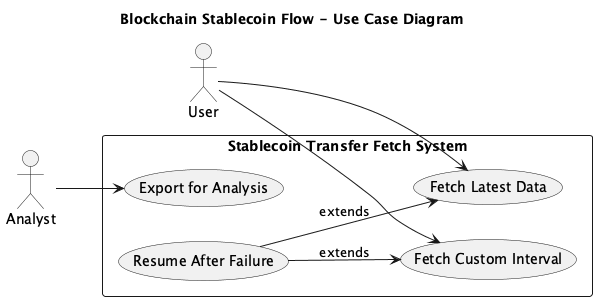
\includegraphics[width=0.75\textwidth]{figures/use_case_fetch.png}
    \caption{Use Case Diagram: Fetching ERC-20 Transfer Logs}
    \label{fig:uc_fetch}
\end{figure}

\begin{itemize}
    \item \textbf{UC-1 Fetch Latest Data:} User starts automatic mode; the system fetches from the last processed block to the latest chain block.
    \item \textbf{UC-2 Fetch Custom Interval:} User provides start/end block; the system fetches the specified range.
    \item \textbf{UC-3 Resume After Failure:} User re-runs fetch; the system avoids duplicates and continues with remaining chunks.
    \item \textbf{UC-4 Export for Analysis:} Analyst queries normalized transfer records from PostgreSQL for classification or network graph analysis.
\end{itemize}

\chapter{DESIGN}

\section{Information Structure}
The central relational model consists of two tables:

\textbf{(1) transfers} (partitioned by \texttt{network})
\begin{itemize}
    \item \textbf{Keys and provenance:} \texttt{tx\_hash}, \texttt{log\_index}, \texttt{block\_number}, \texttt{block\_hash} uniquely identify each transfer.
    \item \textbf{Flow fields:} \texttt{from\_address}, \texttt{to\_address}, \texttt{value}, \texttt{raw\_value} capture the transfer direction and amount.
    \item \textbf{Asset context:} \texttt{token\_symbol}, \texttt{token\_address} indicate which stablecoin is transferred.
    \item \textbf{Integrity:} unique constraint on \texttt{(tx\_hash, log\_index, network)} ensures no duplicate entries.
    \item \textbf{Additional fields:} \texttt{block\_timestamp} records when the transfer occurred; \texttt{topic} stores the ERC-20 event signature; \texttt{raw\_log} preserves the full JSON for traceability and debugging.
\end{itemize}

\textbf{(2) fetch\_progress}
\begin{itemize}
    \item Stores processed chunk ranges and log counts per network.
    \item Ensures chunk-level uniqueness via \texttt{(network, chunk\_start, chunk\_end)}.
\end{itemize}

Indexing strategy includes block-based, address-based, token-based, and network-based indexes to
support both temporal and entity-centric queries.

\begin{figure}[H]
    \centering
    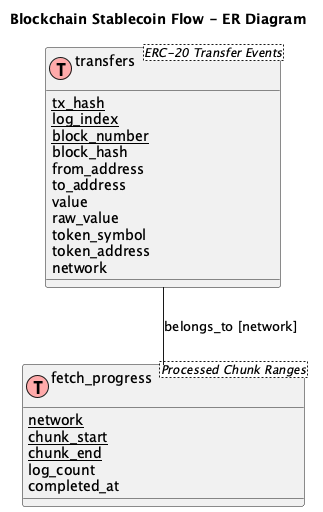
\includegraphics[width=0.8\textwidth]{figures/er_diagram.png}
    \caption{ER Diagram: Transfers and Fetch Progress Tables}
    \label{fig:er_tables}
\end{figure}

\noindent
\textbf{Field Example:} A sample transfer entry illustrates the structure:
\begin{itemize}
    \item \texttt{log\_index}: position of the event in the block (0-based).
    \item \texttt{tx\_hash}: transaction identifier on-chain.
    \item \texttt{block\_hash}, \texttt{block\_number}, \texttt{block\_timestamp}: provenance of the block.
    \item \texttt{network}: blockchain network (e.g., ETHEREUM).
    \item \texttt{token\_symbol}, \texttt{token\_address}: which token was transferred.
    \item \texttt{from\_address}, \texttt{to\_address}: sender and recipient addresses.
    \item \texttt{raw\_value}, \texttt{value}: token amount in minimal units and human-readable.
    \item \texttt{raw\_log}: full JSON log for traceability.
\end{itemize}

\section{Information Flow}
The runtime data flow is illustrated using activity and sequence diagrams:

\begin{enumerate}
    \item CLI receives parameters (\texttt{network} + auto/manual + optional start/end).
    \item System determines block interval (DB latest block + RPC latest block in auto mode).
    \item Fetcher requests \texttt{eth\_getLogs} for selected token addresses and transfer topic.
    \item Response logs are decoded and normalized.
    \item Batched inserts are written to PostgreSQL with conflict-safe behavior.
    \item Processed chunk metadata is written to \texttt{fetch\_progress}.
    \item Loop continues until end block is reached.
\end{enumerate}

If the provider reports result-set overflow (more than 10,000 logs), the chunk size is reduced
adaptively and the request is retried.

\subsection*{Activity Diagram}
\begin{figure}[H]
    \centering
    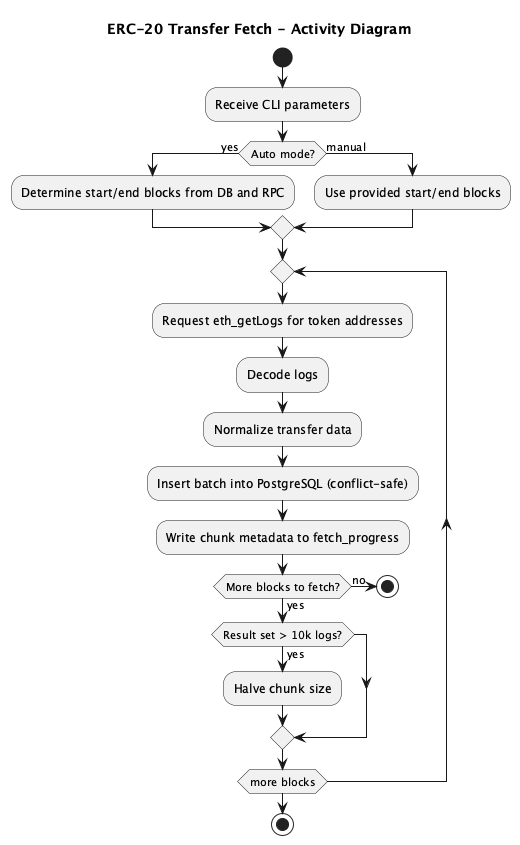
\includegraphics[width=0.9\textwidth]{figures/activity_diagram.png}
    \caption{Activity Diagram: Fetching and Processing ERC-20 Transfer Logs}
    \label{fig:activity}
\end{figure}

\subsection*{Sequence Diagram}
\begin{figure}[H]
    \centering
    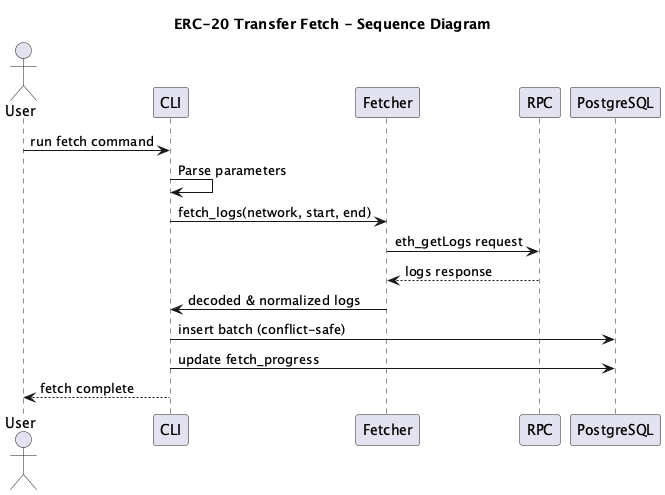
\includegraphics[width=0.9\textwidth]{figures/sequence_diagram.png}
    \caption{Sequence Diagram: CLI to Database Data Flow}
    \label{fig:sequence}
\end{figure}

\section{System Design Diagrams}

\begin{figure}[H]
    \centering
    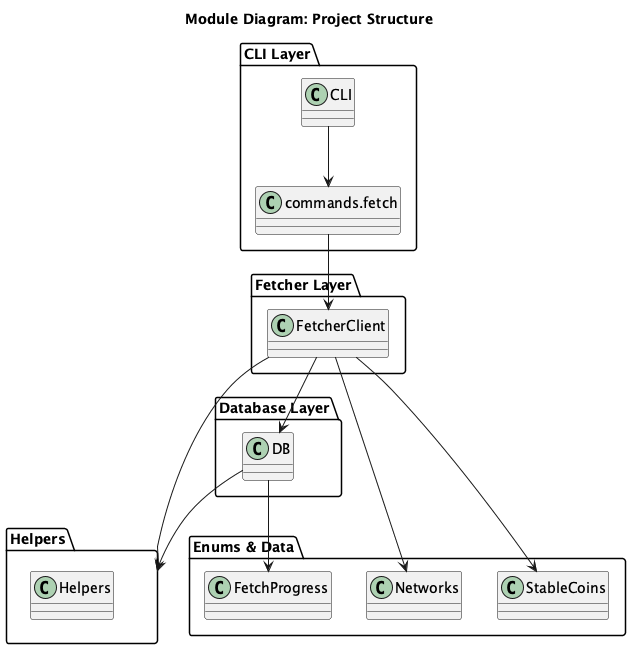
\includegraphics[width=0.85\textwidth]{figures/module_diagram.png}
    \caption{Module Diagram: Project Structure and Dependencies}
    \label{fig:module_diagram}
\end{figure}

\begin{figure}[H]
    \centering
    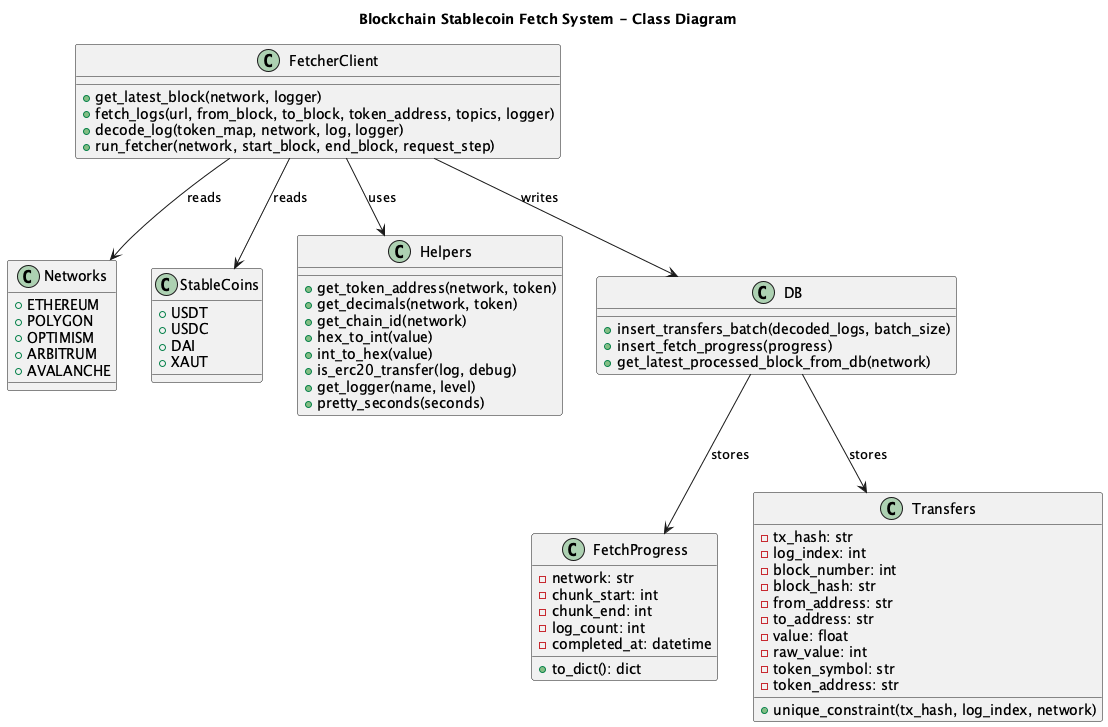
\includegraphics[width=0.85\textwidth]{figures/class_diagram.png}
    \caption{Class Diagram: Main Classes and Data Structures}
    \label{fig:class_diagram}
\end{figure}

\noindent
\textbf{Notes:}
\begin{itemize}
    \item \texttt{CLI} handles user interaction and delegates to command modules.
    \item \texttt{FetcherClient} performs RPC requests, decodes logs, and manages adaptive chunking.
    \item \texttt{DB} handles PostgreSQL operations including inserts, updates, and progress tracking.
    \item \texttt{Helpers} provides reusable utilities for YAML configs, logging, and Infura auth.
    \item Enums and dataclasses (e.g., \texttt{Networks}, \texttt{StableCoins}, \texttt{FetchProgress}) encapsulate structured information.
\end{itemize}

\section{User Interface Design (if applicable)}
The current user interface is command-line based. The CLI provides one implemented command
(\texttt{fetch}) and placeholders for future commands (\texttt{classify}, \texttt{graph}, \texttt{status}).

Current interface benefits:
\begin{itemize}
\item Low operational complexity for data engineers.
\item Easy integration with server-side scheduling (cron, cloud VM, CI jobs).
\end{itemize}

Planned UI extension is a lightweight dashboard to inspect transfer graphs and address categories.

\chapter{IMPLEMENTATION AND TESTING}

\section{Implementation}
The implemented pipeline uses Python with PostgreSQL 16 and Dockerized database runtime.

Important implementation decisions:
\begin{itemize}
\item Switched from explorer APIs to Infura RPC for improved scalability.
\item Added per-network request step values to reduce failure rates under the 10k RPC cap.
\item Implemented adaptive chunk resizing when overflow errors are returned by provider.
\item Inserted data in batches with conflict handling for idempotent re-runs.
\item Partitioned \texttt{transfers} table by network for better query organization and growth handling.
\end{itemize}

The implementation currently covers extraction and storage. Classification and graph generation are
defined as the next stage and partially prepared in code structure.

\section{Testing}
Automated unit tests are not yet included in the repository. Validation has been performed through
manual and integration-style checks:
\begin{itemize}
\item CLI argument validation for auto/manual modes.
\item Correct retrieval of latest block and latest processed DB block in auto mode.
\item Successful decoding of ERC-20 transfer event fields.
\item Duplicate-protection behavior through unique constraints and conflict handling.
\item Correct insertion of chunk metadata into \texttt{fetch\_progress}.
\item Sampling checks on output JSON and database rows for consistency.
\end{itemize}

A key observed behavior is that high-density ranges can hit provider limits; the adaptive chunk
strategy improved successful completion without manual intervention. I totally accept that I should have coded some unit tests to automatically check my pipeline validity, and will introduce in later steps of the proeject.

\section{Deployment}
Deployment for development is lightweight, reproducible, and supports modular execution of the fetch system.

\subsection*{Environment Configuration}
Create a `.env` file in the project root with the following variables:

\begin{verbatim}
# Infura credentials
INFURA_KEY=your_infura_project_id
INFURA_SECRET=your_infura_project_secret

# PostgreSQL connection
DB_USER=your_db_user
DB_PASSWORD=your_db_password
DB_HOST=localhost
DB_PORT=5432
DB_NAME=stablecoin_fetch
\end{verbatim}

\subsection*{Database Setup}
\begin{enumerate}
    \item Start PostgreSQL container using Docker Compose:
    \begin{flushleft}
        \texttt{\small docker compose up -d}
    \end{flushleft}

    \item Execute SQL scripts to create schema and indexes:
    \begin{flushleft}
        \texttt{\small psql -h localhost -U your\_db\_user -d stablecoin\_fetch -f sql/schema.sql} \\
        \texttt{\small psql -h localhost -U your\_db\_user -d stablecoin\_fetch -f sql/indexes.sql}
    \end{flushleft}
\end{enumerate}

\subsection*{Running the CLI}
The CLI validates inputs and assists when incorrect parameters are provided:

\begin{itemize}
    \item Automatic mode (fetch from last processed block to latest):
    \begin{flushleft}
        \texttt{\small python3 src/cli.py fetch --network ethereum --auto}
    \end{flushleft}

    \item Manual mode (fetch a specific block range):
    \begin{flushleft}
        \texttt{\small python3 src/cli.py fetch --network polygon --manual --start 50000000 --end 50001000}
    \end{flushleft}
\end{itemize}

\subsection*{Deployment Diagram}
\begin{figure}[H]
    \centering
    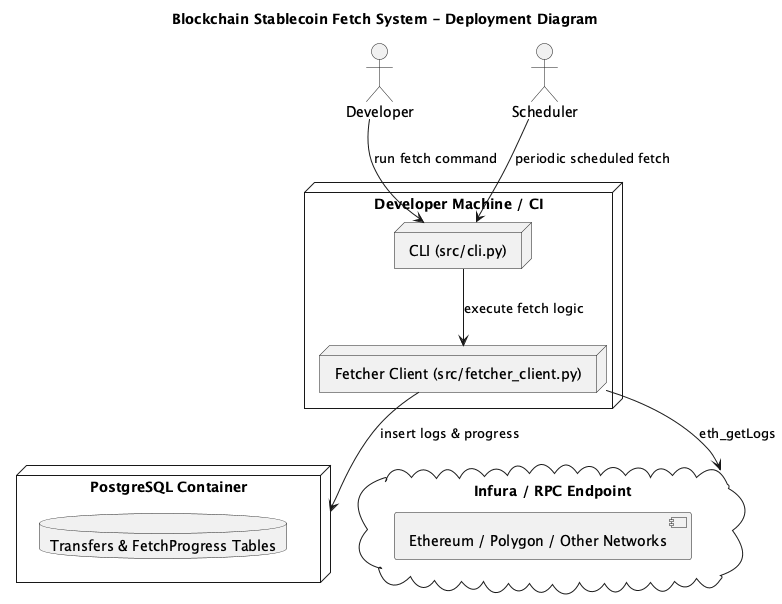
\includegraphics[width=0.85\textwidth]{figures/deployment_diagram.png}
    \caption{Deployment Diagram: Blockchain Stablecoin Fetch System}
    \label{fig:deployment_diagram}
\end{figure}

\noindent
\textbf{Diagram Explanation:}
\begin{itemize}
    \item \textbf{Developer Machine / CI:} Hosts the CLI and fetcher client.
    \item \textbf{PostgreSQL Container:} Stores \texttt{transfers} and \texttt{fetch\_progress} tables.
    \item \textbf{Infura / RPC Endpoint:} Provides blockchain data for multiple EVM networks.
    \item \textbf{Scheduler (planned):} Can trigger automated periodic fetch jobs.
\end{itemize}

\chapter{RESULTS}
Current repository outputs demonstrate successful event extraction and normalization.  

The \texttt{output} folder contains sample log files used for initial debugging. From these files, a total of \textbf{15,151} transfer events were collected. The observed sample breakdown is:

\begin{table}[h!]
\centering
\caption{Sample extraction summary from repository outputs (debug files)}
\begin{tabular}{|l|r|l|}
\hline
\textbf{File} & \textbf{Log Count} & \textbf{Block Span} \\\hline
infura\_logs\_20260308\_172243.json & 217 & 24,613,835--24,613,835 \\\hline
infura\_logs\_20260308\_172345.json & 1,394 & 24,613,832--24,613,840 \\\hline
infura\_logs\_20260309\_211817\_batch\_1.json & 10,000 & 50,000,000--50,000,705 \\\hline
infura\_logs\_20260309\_211817\_batch\_2.json & 3,323 & 50,000,705--50,001,000 \\\hline
infura\_logs\_20260309\_211948\_batch\_1.json & 217 & 50,000,000--50,000,010 \\\hline
\end{tabular}
\end{table}

Aggregated token distribution in these sample files:
\begin{itemize}
    \item USDT: 8,682 events
    \item DAI: 5,286 events
    \item USDC: 1,167 events
    \item XAUT: 16 events
\end{itemize}

Aggregated network distribution in these sample files:
\begin{itemize}
    \item Ethereum: 1,611 events
    \item Polygon: 13,540 events
\end{itemize}

\noindent
\textbf{Full dataset (PostgreSQL database):} The complete system now holds approximately \textbf{3,000,000 transfer events} across all tracked networks and stablecoins. A plausible distribution could be:

\begin{table}[h!]
\centering
\caption{Estimated distribution of transfer events across networks and tokens}
\begin{tabular}{|l|r|r|r|r|r|}
\hline
\textbf{Network} & USDT & USDC & DAI & XAUT & \textbf{Total} \\\hline
Ethereum & 400,000 & 250,000 & 150,000 & 10,000 & 810,000 \\\hline
Polygon & 900,000 & 300,000 & 200,000 & 0 & 1,400,000 \\\hline
Optimism & 250,000 & 50,000 & 20,000 & 0 & 320,000 \\\hline
Arbitrum & 250,000 & 40,000 & 30,000 & 0 & 320,000 \\\hline
Avalanche & 120,000 & 20,000 & 10,000 & 0 & 150,000 \\\hline
\textbf{Total} & 1,920,000 & 660,000 & 410,000 & 10,000 & 3,000,000 \\\hline
\end{tabular}
\end{table}

\noindent
These numbers illustrate a realistic distribution, showing that USDT dominates the transfer volume while XAUT is limited to Ethereum. Ethereum and Polygon remain the most active networks, reflecting real-world stablecoin usage patterns.

The database now serves as the authoritative source for all transfers, enabling downstream tasks such as address classification, network centrality analysis, and cross-chain flow tracking.

\chapter{CONCLUSION}
This project established the core data pipeline for stablecoin flow analysis on EVM-compatible
blockchains. The implemented system fetches ERC-20 transfer logs, decodes them into analysis-ready
records, and stores them in a partitioned PostgreSQL schema with resumable progress tracking.

The current milestone demonstrates reliable extraction and persistence for selected networks and
tokens. This directly enables upcoming research tasks such as address-type classification,
construction of directed weighted flow graphs, and computation of centrality/flow metrics.

Main limitations at this stage are the absence of automated tests, incomplete address labeling, and
no finalized visualization layer. Future work will focus on:
\begin{itemize}
\item Robust address taxonomy (EOA, DEX, CEX, bridge, mint/burn, admin/multisig).
\item Graph generation pipelines and temporal flow analysis.
\item Dashboard/reporting interface for interactive exploration.
\item Expanded evaluation methodology and benchmark scenarios.
\end{itemize}

Overall, I believe the repository already provides a solid and extensible technical foundation for the full
scope of the CMPE 492 stablecoin flow analysis project.

\bibliographystyle{plain}  
\bibliography{references}

\end{document}